% begin Chapter ResearchEvaluation

\chapter {Research Evaluation}
\label{chapter-ResearchEvaluation}

\paragraph {} In the previous chapter, we took a look at the proposed system architecture and it's features. We also understood what the entities in the system were and how they relate to each other. In any research, the evaluation of the concept is as, if not more, important to the justifying the end result. Accordingly an evaluation of the prototype was carried out with the schedulers and the commuters.



\section{User Evaluation of Prototype}

\paragraph{} There are 3 main types of users that used this research prototype. They are,

\begin{itemize}
\item Schedulers of the Transport Authority
\item Commuters
\item Bus Owners and Operators
\end{itemize}

\paragraph{} Of these 3 main types of users, the Schedulers act as the Admins and they can carry out the Admin functionalities listed under Section~\ref{systemFeatures}. Each of these users will have different views and functionalities associated with them. The User evaluation was carried out only with the Schedulers and the Commuters as I was unable to find any Bus Owners / Operators willing to participate in this study.

The prototype was hosted on a free hosting service and the Schedulers were interviewed while they were using the system to obtain a qualitative feedback on the prototype and its functionality. The URL of the public interface was sent to regular commuters to ascertain their feedback on the system. The prototype system can be accessed at \url{http://gaman.byethost4.com/}.


\subsection{Feedback of the Schedulers}

\paragraph{} The feedback from the schedulers was overwhelmingly positive towards the system. They said they welcome a system like this and would gladly use it if it does eventually become a system ready for implementation. Furthermore, they mentioned that the User Interface was very simple, easy-to-use and intuitive.

The Schedulers also pointed out that an implementable system would need some added functionality such as the ability to store timetables, generate timetables automatically when given the data and the vehicle and crew scheduling functionalities. However, they said as this is a prototype system, the concept is correct, sound and suitable for further development. (Source: Interviews with the Scheduling Officers of the WP RPTA)


\subsection{Feedback of the Commuters}

\paragraph{} After hosting the prototype online, a group of commuters were provided the link and given an explanation on how to use the system. Then they were asked to fill out a survey on their experience using the Gaman prototype system. The key points have been summarized and the results have been tabulated below. The Survey can be accessed at the following URL: \url{https://docs.google.com/forms/d/100pWQ4476Mo4tqn3SHLmVO1r8cB-ayuQEdai8xWyjCI/viewform/}

\begin {itemize}

\item Number of Participants: 39

\item Age group - Table~\ref{table-survey-ageGroupOfSurveyParticipants}

\begin{table} [H]
\centering
\begin{tabular}{|l|c|}
\hline
Age Group & Number of participants \\
\hline
20-35	&38 \\
10-19	&01 \\
\hline
\end{tabular}
\caption{Age Groups of Participants}
\label{table-survey-ageGroupOfSurveyParticipants}
\end{table}

\item Frequency of travel in the bus - Table~\ref{table-survey-frequencyOfTravelInTheBus}

\begin{table} [H]
\centering
\begin{tabular}{|l|c|}
\hline
Frequency of travel & Number of participants \\
\hline
Daily, one or two times a day	&20 \\
Daily, several times a day	&15 \\
A few times a week	&03 \\
A few times a month	&01 \\
\hline
\end{tabular}
\caption{Frequency of travel in the bus}
\label{table-survey-frequencyOfTravelInTheBus}
\end{table}



\item Rating - Information Portal (Scale of 1 to 5 with 5 being "Very Useful" and 1 being "Not useful at all") - Table~\ref{table-survey-rating-InformationPortal} - Figure~\ref{image-ratingInformationPortal}

\begin{table} [H]
\centering
\begin{tabular}{|l|c|}
\hline
Rating & Number of participants \\
\hline
5	&09 \\
4	&20 \\
3	&07 \\
2	&03 \\
1	&00 \\
\hline
\end{tabular}
\caption{Rating - Information Portal}
\label{table-survey-rating-InformationPortal}
\end{table}

\begin {figure} [H]
\centering
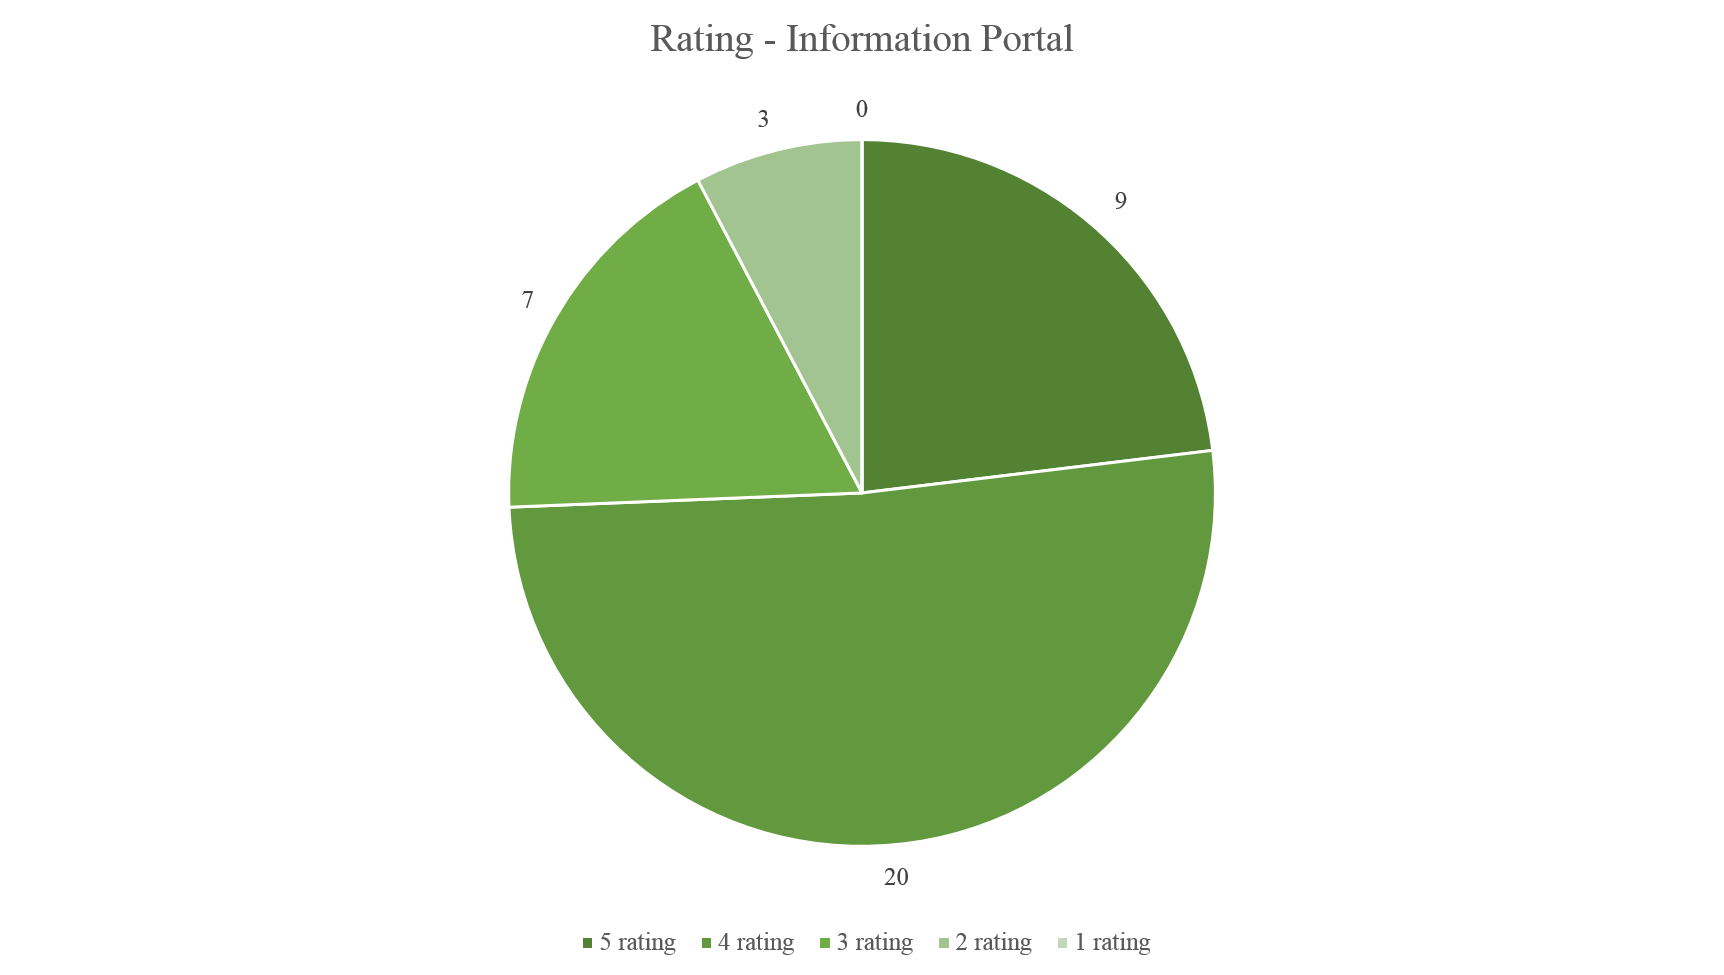
\includegraphics [scale=0.7] {ratingInformationPortal}
\caption [Chart - Rating - Information Portal] {Chart - Rating - Information Portal}
\label {image-ratingInformationPortal}
\end {figure}

\item Qualitative comments received
\begin {itemize}
\item "well i think infomation about bus routes is useful if we want to travel to a place that we dnt know using bus routes. most of the time i use google maps to navigate but it doesnt provide me the functionality of which bus route should i take. so i think this is a good effort"
\item "useful."
\item "It is a superb move. Very informative and useful. Hope this is mobile friendly as well."
\item "Very helpful. There are sufficient information regarding buses and bus routes and personals."
\item "It is great that we can use this system to get information about the buses and owners."
\item "Really good one"
\end {itemize}



\item Rating - Bus Route Finder (Scale of 1 to 5 with 5 being "Very Useful" and 1 being "Not useful at all") - Table~\ref{table-survey-rating-BusRouteFinder} - Figure~\ref{image-ratingBusRouteFinder}

\begin{table} [H]
\centering
\begin{tabular}{|l|c|}
\hline
Rating & Number of participants \\
\hline
5	&12 \\
4	&16 \\
3	&09 \\
2	&02 \\
1	&01 \\
\hline
\end{tabular}
\caption{Rating - Bus Route Finder}
\label{table-survey-rating-BusRouteFinder}
\end{table}

\begin {figure} [H]
\centering
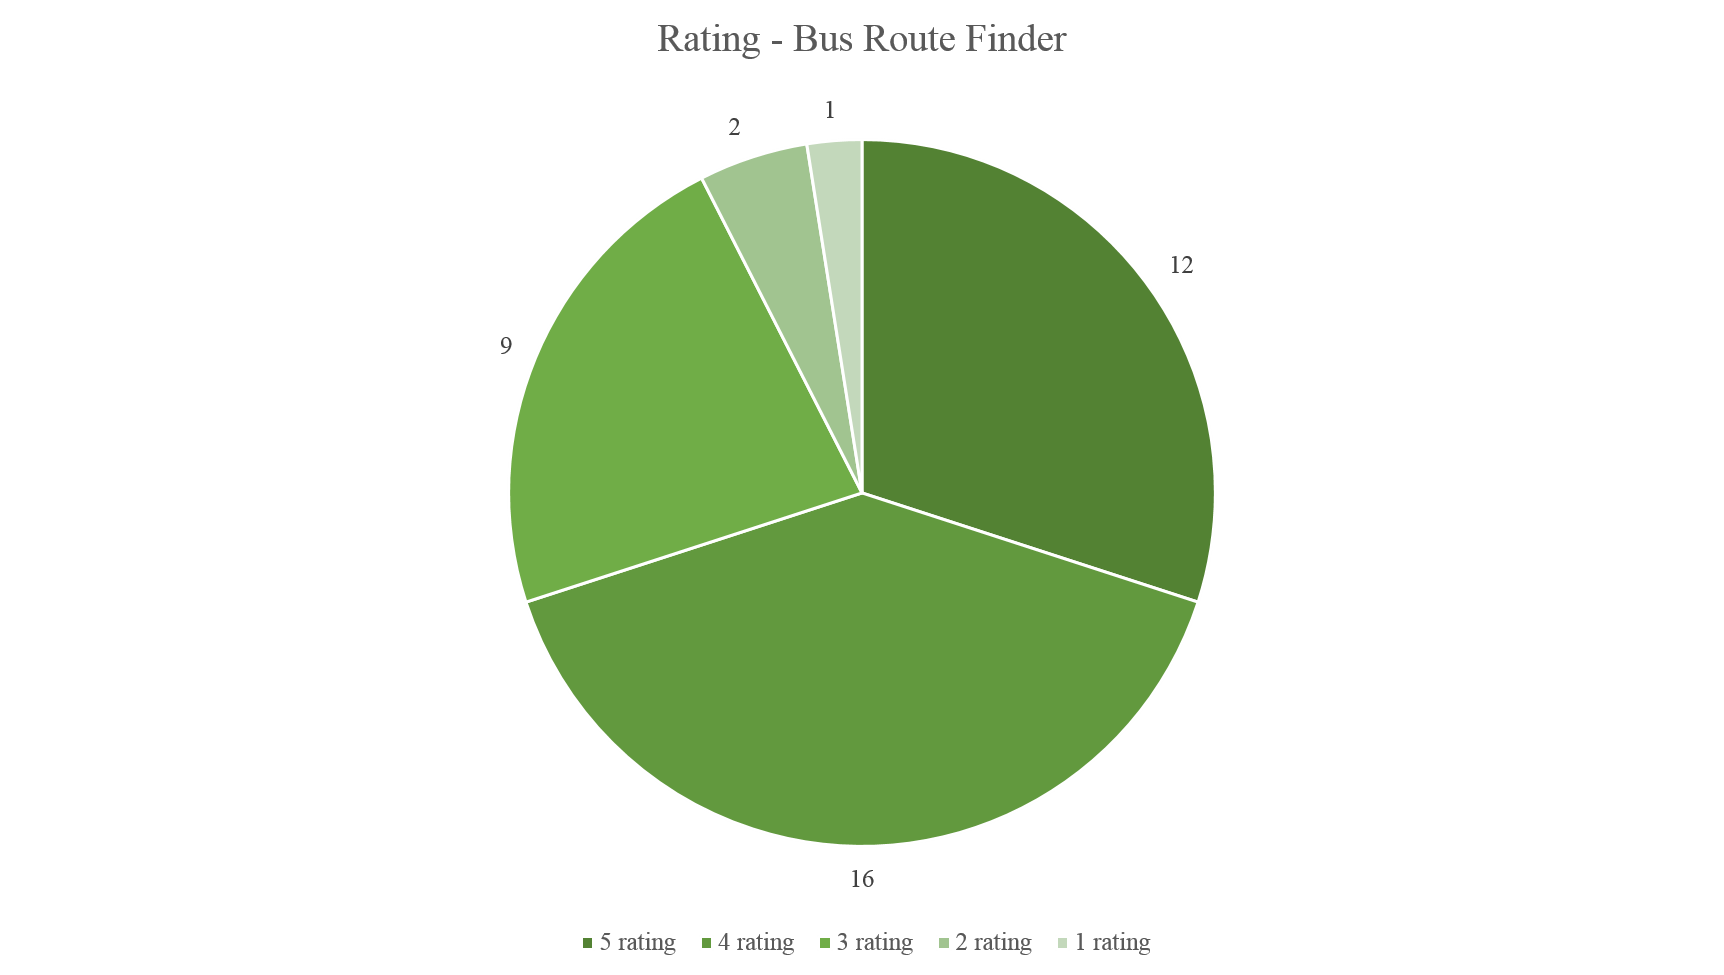
\includegraphics [scale=0.7] {ratingBusRouteFinder}
\caption [Chart - Rating - Bus Route Finder] {Chart - Rating - Bus Route Finder}
\label {image-ratingBusRouteFinder}
\end {figure}

\item Qualitative comments received
\begin {itemize}
\item "simple but effective solution to easily find the routes."
\item "It's better if the information were presented in a better way, so that those can be found easily (E.g. provide searching facilities etc.)"
\item "More places need to be added to the system. It's better to give the bus route with the start and end destination as the first details. for some users sometimes giving only route number will not make sense very much."
\end {itemize}



\item Rating - Feedback Functionality (Scale of 1 to 5 with 5 being "Very Useful" and 1 being "Not useful at all") - Table~\ref{table-survey-rating-FeedbackFunctionality} - Figure~\ref{image-ratingFeedbackFunctionality}

\begin{table} [H]
\centering
\begin{tabular}{|l|c|}
\hline
Rating & Number of participants \\
\hline
5	&09 \\
4	&14 \\
3	&13 \\
2	&03 \\
1	&00 \\
\hline
\end{tabular}
\caption{Rating - Feedback Functionality}
\label{table-survey-rating-FeedbackFunctionality}
\end{table}

\begin {figure} [H]
\centering
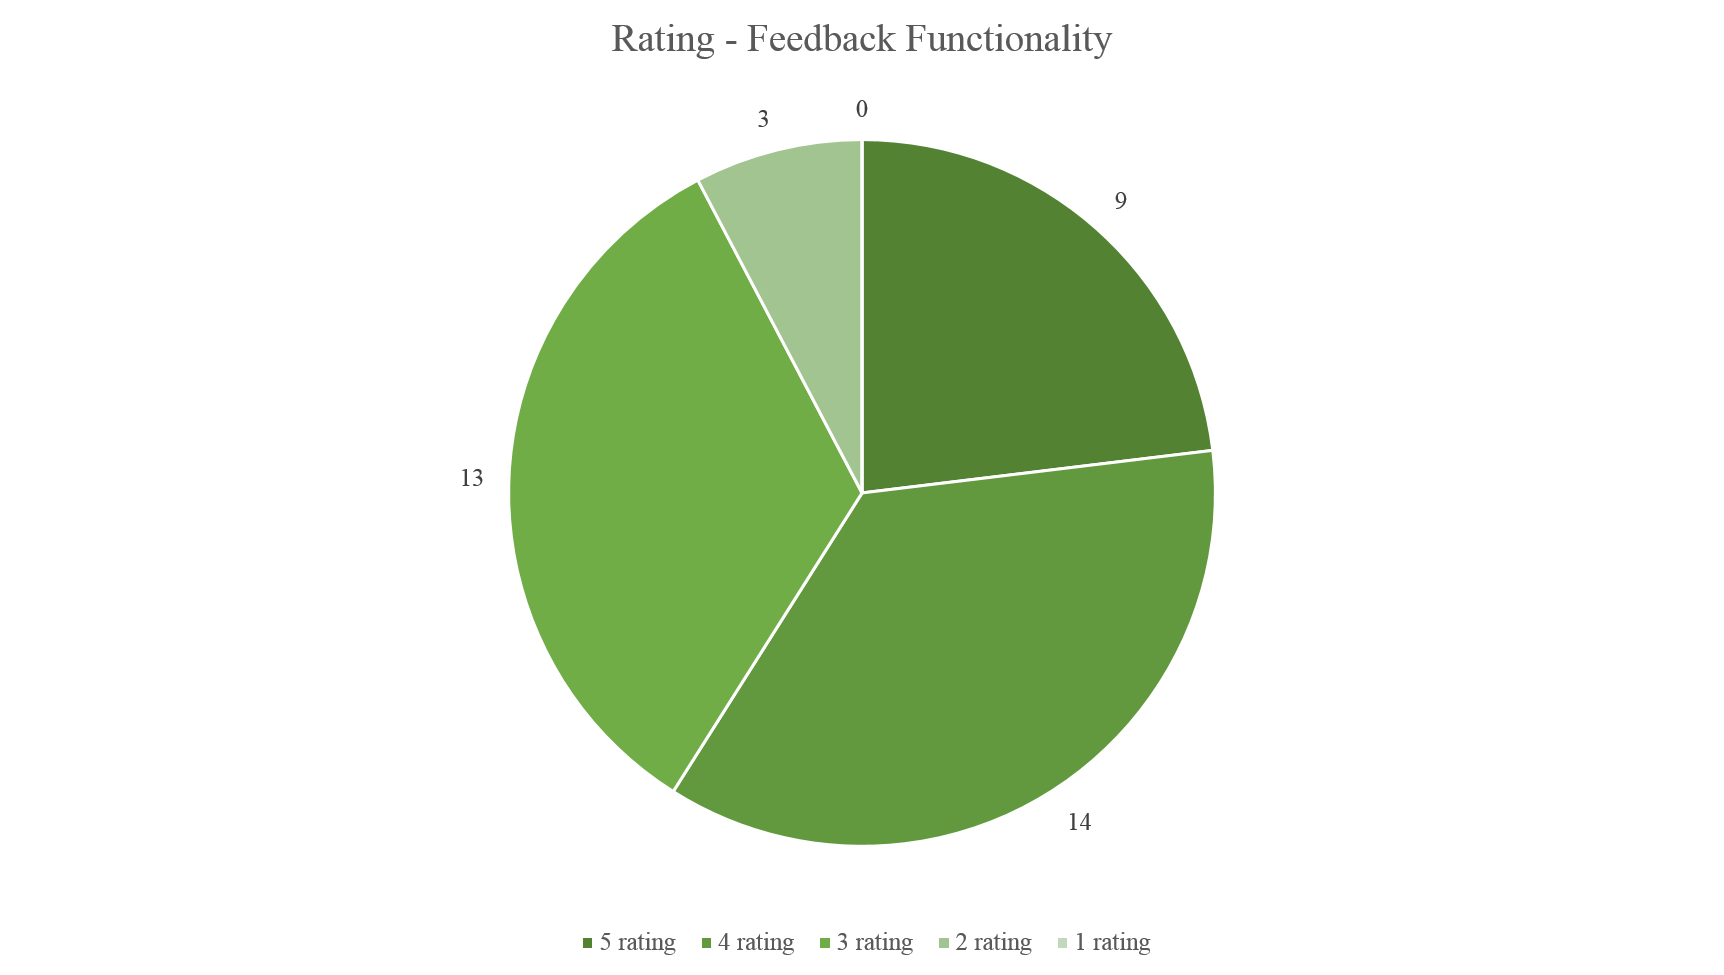
\includegraphics [scale=0.7] {ratingFeedbackFunctionality}
\caption [Chart - Rating - Feedback Functionality] {Chart - Rating - Feedback Functionality}
\label {image-ratingFeedbackFunctionality}
\end {figure}

\item Qualitative comments received
\begin {itemize}
\item "Needs the ability to connect drivers and conductors to buses,feedbacks and complaints. drivers and conducters may get assigned to the buses by a time table component. ( couldn't test this since i couldn't see the needed form elements for filling those info while giving feedback )"
\item "Feedback to drivers and conductors may not reach them because of the low computer literacy. However, if there is any responsible person to handle or communicate with them then it is really useful function"
\end {itemize}



\item Rating - Comlaints Functionality (Scale of 1 to 5 with 5 being "Very Useful" and 1 being "Not useful at all") - Table~\ref{table-survey-rating-ComplaintsFunctionality} - Figure~\ref{image-ratingComplaintsFunctionality}

\begin{table} [H]
\centering
\begin{tabular}{|l|c|}
\hline
Rating & Number of participants \\
\hline
5	&08 \\
4	&16 \\
3	&10 \\
2	&05 \\
1	&00 \\
\hline
\end{tabular}
\caption{Rating - Complaints Functionality}
\label{table-survey-rating-ComplaintsFunctionality}
\end{table}

\begin {figure} [H]
\centering
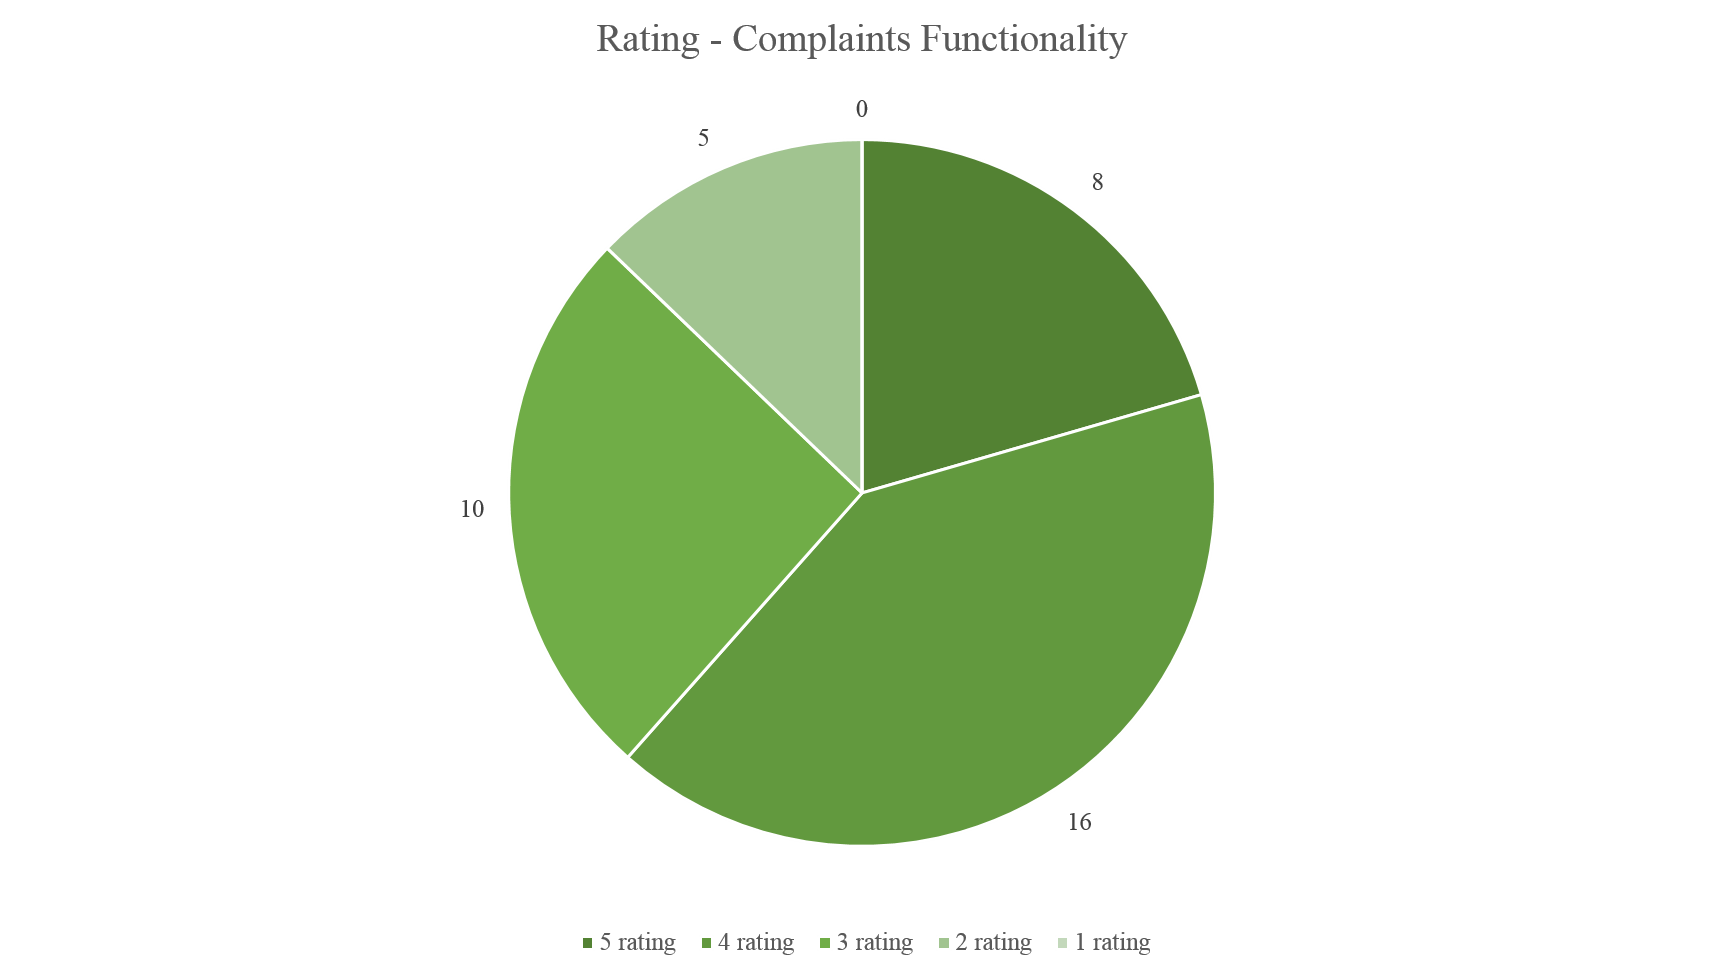
\includegraphics [scale=0.7] {ratingComplaintsFunctionality}
\caption [Chart - Rating - Complaints Functionality] {Chart - Rating - Complaints Functionality}
\label {image-ratingComplaintsFunctionality}
\end {figure}

\item Qualitative comments received
\begin {itemize}
\item "This is a very useful functionality that would help in increasing and maintaining the quality of the bus services."
\item "This is really good because sometimes we have to bare all the sh***y experiences or will be able to share it with few friends and forget about those. But this functionality facilitates us to share our good/bad experiences with others and even will be able to do something."
\item "It's very useful to have such functionality, because that is one of  the main problem we can see in the public transport system in Sri Lanka."
\item "I wish the complain data were more specific. For example, user might be interested in knowing the bus-route associated with a certain complain or he might be interested viewing all the complains related to a certain but-route."
\item "If it functioned properly this will have a big impact. Simply a user can share their own experience. But there are possibilities of fake complaints."
\end {itemize}



\item Rating - User Interface (Scale of 1 to 5 with 5 being "Very easy to use" and 1 being "Very difficult to use") - Table~\ref{table-survey-rating-UserInterface} - Figure~\ref{image-ratingUserInterface}

\begin{table} [H]
\centering
\begin{tabular}{|l|c|}
\hline
Rating & Number of participants \\
\hline
5	&16 \\
4	&11 \\
3	&09 \\
2	&02 \\
1	&01 \\
\hline
\end{tabular}
\caption{Rating - User Interface}
\label{table-survey-rating-UserInterface}
\end{table}

\begin {figure} [H]
\centering
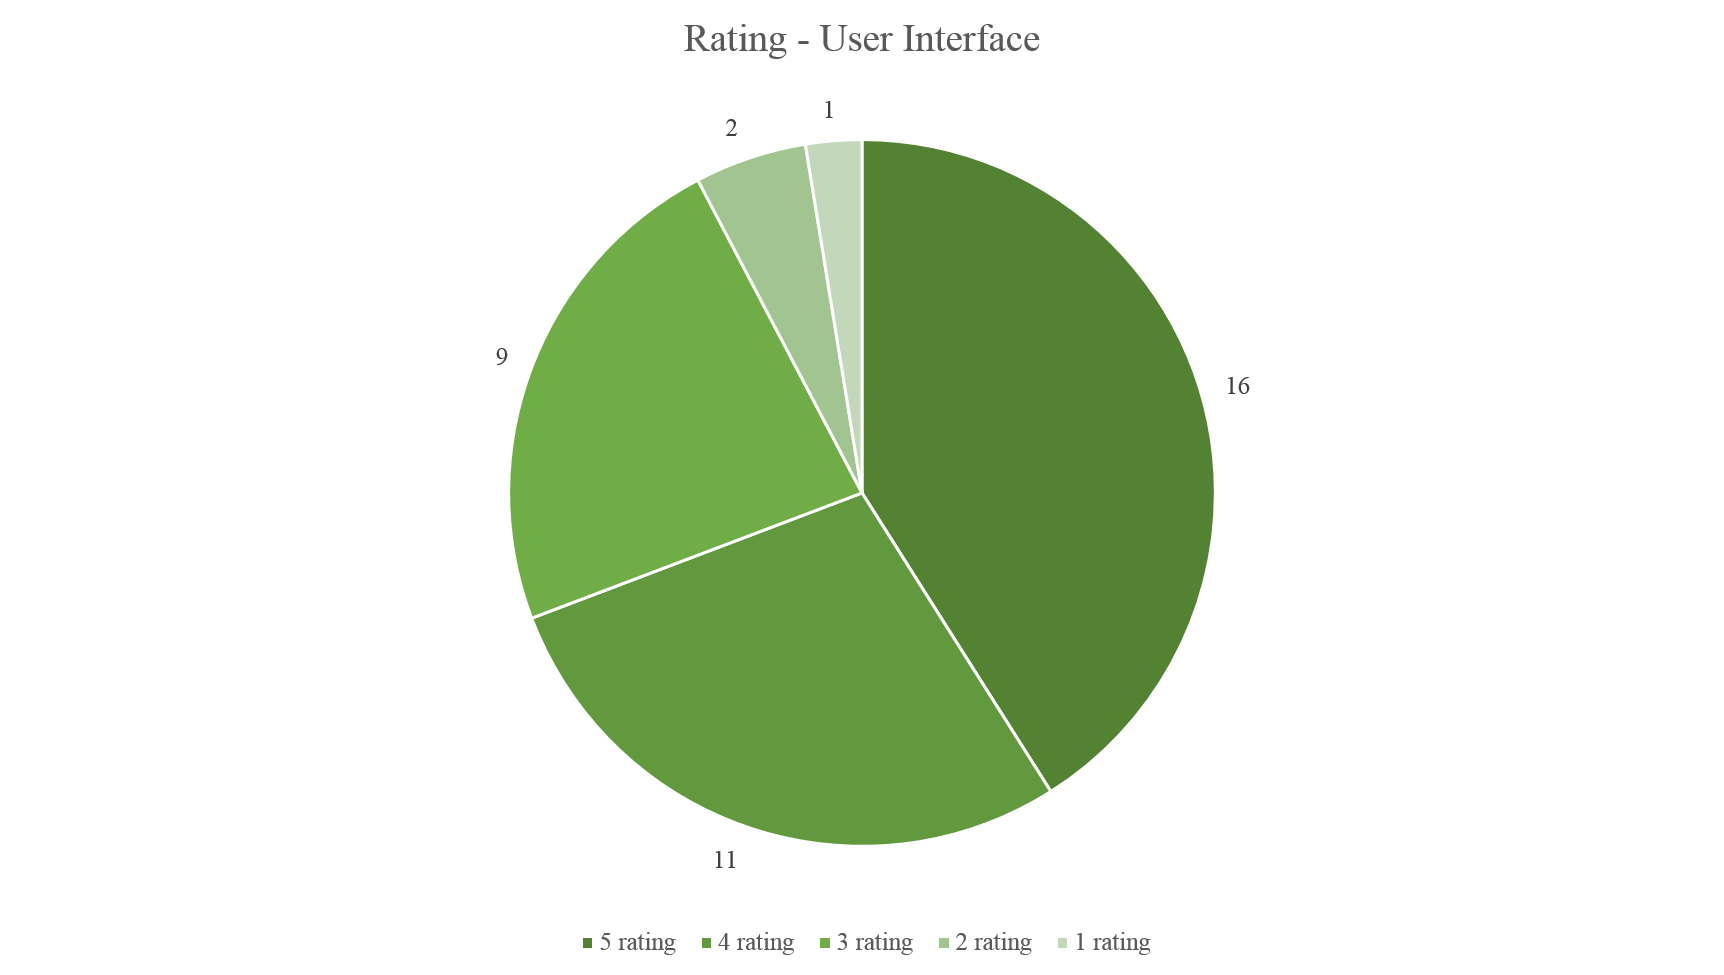
\includegraphics [scale=0.7] {ratingUserInterface}
\caption [Chart - Rating - User Interface] {Chart - Rating - User Interface}
\label {image-ratingUserInterface}
\end {figure}

\item Qualitative comments received
\begin {itemize}
\item "good. but can improve. trade off between simplicity and ease of use."
\item "Simple and nice! good work!"
\item "Simple, but effective and attractful. Nicely developed."
\item "Looks a bit too linear in my opinion... more vibrant colours should be used to highlight the important and most frequently used features.."
\item "I like the simplest interface and colors. Some pages have textboxes whichs seems very small comparing to the screen size. Better if you add some autoresize them"
\end {itemize}



\item Survey Question - Would you use a system like this if it was implemented? - Table~\ref{table-survey-question-WouldYouUseASystemLikeThis} - Figure~\ref{image-questionWouldYouUse}

\begin{table} [H]
\centering
\begin{tabular}{|l|c|}
\hline
Rating & Number of participants \\
\hline
Oh my god, yes!	&16 \\
Yes	&17 \\
No	&06 \\
\hline
\end{tabular}
\caption{Survey Question - Would you use a system like this if it was implemented?}
\label{table-survey-question-WouldYouUseASystemLikeThis}
\end{table}

\begin {figure} [H]
\centering
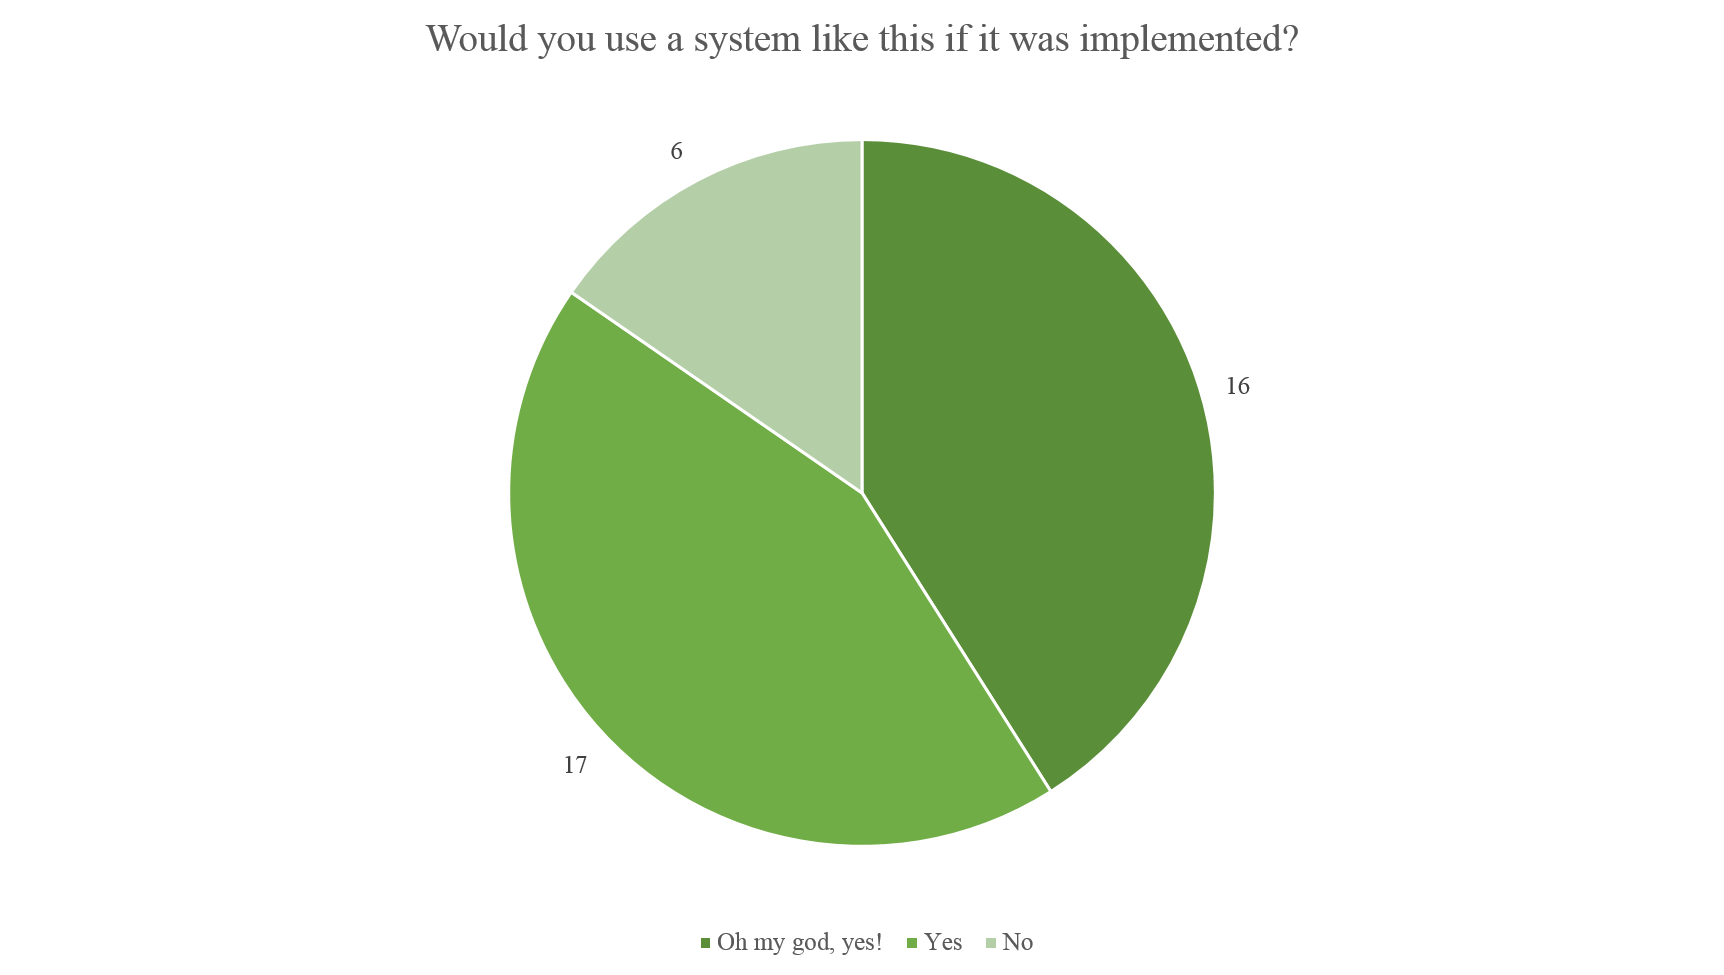
\includegraphics [scale=0.7] {questionWouldYouUse}
\caption [Chart - Survey Question] {Chart - Survey Question}
\label {image-questionWouldYouUse}
\end {figure}

\end {itemize}



\section{Literature Published related to this Research Project}

\paragraph{} A research paper on the work related to this research project was submitted to the 2013 European, Mediterranean \& Middlle-eastern Conference on Information Systems (EMCIS). The paper was accepted subject to changes. The paper was an analysis of trasnportation systems in developing countries and how an Information Systems solution would help solve the problems faced in the public transportation domain. The details of the paper are listed below.

\begin {itemize}
\item Title: "A Transportation Management Information System for Public Transport in Developing Countries."
\item Authors: Aftha Jaldin and Dr. Shiromi Arunatileka.
\item Abstract: Public Transportation Management in developing countries presents a more challenging environment than its counterpart in developed nations. And, as in any Public Transport System, the Scheduling Process provides the framework in which the Transport Service operates. It is responsible for the formulation of timetables, vehicle and crew scheduling, and crew rostering. Although this is the most important part of the transport system, it is the most difficult to manage. The varied inputs to the process, the lack of proper infrastructure and improper technology and processes available all lead to a unique problem in terms of Public Transportation Management in a developing country. Therefore it is imperative for a system to cater to these limitations and meet the demands of a developing country specifically. Therefore, this paper proposes an alternative system to aid the Schedulers in their capacity to formulate timetables and schedule vehicles and crew. The system will also act as an information portal to commuters to obtain information about transport modes and associated routes as well as other related information. The paper uses the case of the Western Province Bus Transportation System in Sri Lanka as an example to draw conclusions regarding the proposed information system.
\end {itemize}


